\documentclass{article}
\usepackage{graphicx} % Required for inserting images
\usepackage{float}
\usepackage{amsmath}
\usepackage[left=3cm, right=3cm, top=3cm, bottom=3cm]{geometry}
\usepackage[makeroom]{cancel}
\usepackage{booktabs}
\usepackage{comment}
\usepackage{animate}


\setlength{\parindent}{0pt}
\setlength{\parskip}{\baselineskip}

\begin{document}

\hyphenpenalty=10000
\exhyphenpenalty=10000
% Title section
\begin{center}
    \vspace*{4cm}
    
    \large NBE-E4260 Genesis and Analysis of Brain Signals \\
    \vspace{0.5cm}
    
    \LARGE\textbf{Kuramoto Modelling with Desynchronisation}  \\
        
    \vspace{4cm}

    \large Sebastian Hannula \& Martin Häggblom\\

    \today
    
\end{center}
\thispagestyle{empty}
\newpage
\tableofcontents
\newpage
\setcounter{page}{1}

\section{Introduction}

\subsection{Background \& Significance}
Synchronization of globally coupled limit cycle oscillators has raised an interest in a wide variety of fields such as semiconductor laser arrays, cardiac pacemaker cells, and demand-controlled brain pacemakers for the therapy of neurological and psychiatric diseases. The Kuramoto model is one attempt to define these types of complex mechanisms. It describes general properties of the phase dynamics of systems with nonlinear limit cycle oscillators with weak global coupling \cite{Maistrenko}.

Despite studies, the desynchronization mechanism is still far from being clarified in the Kuramoto model \cite{Maistrenko}. Prior art includes; qualitative approaches \cite{Maistrenko}, statistical techniques \cite{Strogatz}, time-delayed interaction, dephasing through chaotic rather than periodical oscillators, fast-changing synaptic coupling, noise, and changes of excitability that have been proposed and studied to describe how oscillator systems desynchronize \cite{Han}. In “Generalising the Kuramoto model for the study of neuronal synchronisation in the brain”, \cite{Cumin} the authors investigated a generalization of the standard Kuramoto model for different connective arrangements, time-varying natural frequency, and time-varying coupling strength to better model brain dynamics.

\subsection{Knowledge gap}
State of the art computational models for describing the desynchronization in brains as a result of specific types of plasticity induced by brain stimulation are discussed in \cite{Manos}. Maistrenko and coworkers investigated the desynchronization in Kuramoto models through bifurcation theory and chaos theory \cite{Maistrenko}. To our knowledge desynchronization based on time-varying coupling strengths in the Kuramoto model, such as in the research by Cumin \& Unsworth\cite{Cumin}, has not been studied very extensively in the prior art. 

One problem with studies related to Kuramoto models for describing the desynchronization in brains is that they seem a bit limited. One potential reason for the aforementioned limitation might be that desynchronization in brains as a phenomena differs more than synchronization in brains when compared to other systems where the Kuramoto model has also been studied e.g. semiconductor laser arrays \cite{Maistrenko}. In other words it might be that studies of synchronization in brains have been able to apply findings from other systems not related to the brain, while applying findings from other systems not related to the brain to studies of desynchronization in brains has not been viable. 

Hence further studies on desynchronization based on time-varying coupling strengths in the Kuramoto model could be regarded as incremental research.

\subsection{Questions \& Hypotheses}

The main scientific question this study aims to answer is:
\begin{itemize}
    \item Can desynchronization be induced into Kuramoto model via time-varying coupling strength of 4 oscillators connected to all-to-all configuration?
\end{itemize}

Beside the main scientific question the study aims additionally to answer the following question:
\begin{itemize}
    \item Can the order parameter results for the Kuramoto model with time-varying coupling strength of 4 oscillators connected to all-to-all configuration presented by Cumin \& Unsworth \cite{Cumin} be reproduced?
\end{itemize}

In figure \ref{fig:1} below the framework for how \cite{Cumin} has presented their findings is shown. The multiple different graphs in each of the subplots on the right represent different randomly selected natural frequencies and initial phases.

\begin{figure}[H]
    \centering
    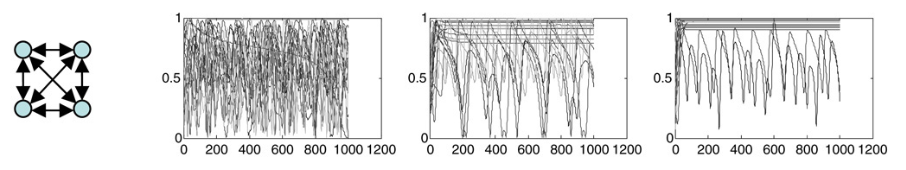
\includegraphics[width=14cm]{Cumin_fig1.png}
    \caption{Four oscillators connected to all-to-all configuration (left) and order parameter results for the Kuramoto model with time-varying coupling strength (right) \cite{Cumin}.}
    \label{fig:1}
\end{figure}

In figure \ref{fig:2} below, the results of interest are shown with characteristic patterns highlighted in blue.

\begin{figure}[H]
    \centering
    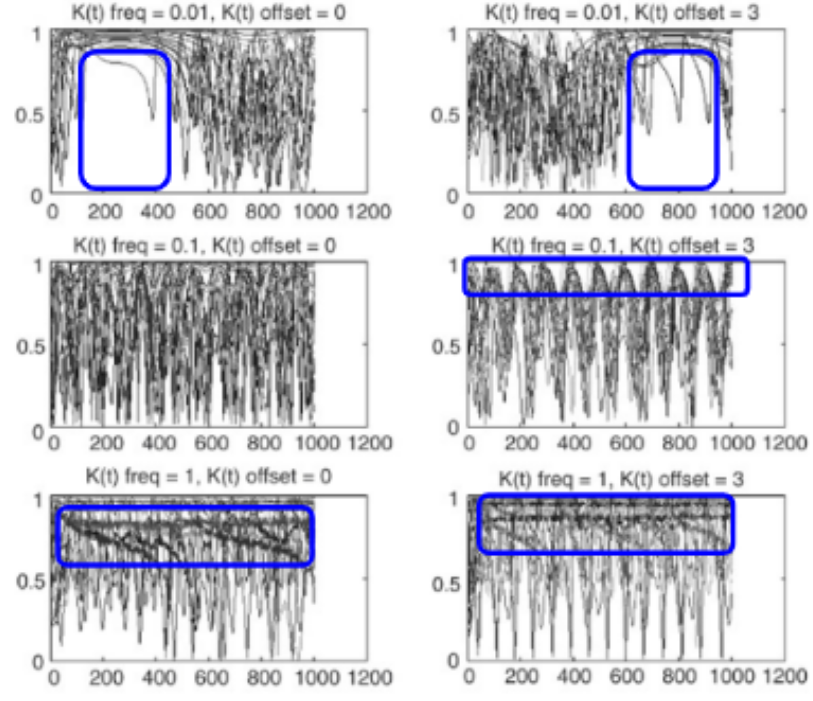
\includegraphics[width=8cm]{Cumin_fig2.png}
    \caption{Order parameter results for time-varying coupling strength Kuramoto model by Cumin \& Unsworth \cite{Cumin}. Blue rectangles have been added in this study in order to indicate which visual characteristics to be compared.}
    \label{fig:2}
\end{figure}

Following hypotheses were formulated to test the main scientific question:
\begin{itemize}
    \item Main H0: There are several peaks in the order parameter for time-varying coupling strength Kuramoto model proving induced desynchronization.
    \item Main H1: There are no peaks. The order parameter for time-varying coupling strength Kuramoto model converges towards synchronization in a similar manner as Kuramoto model.
\end{itemize}

To test the additional question, following hypotheses was constructed:
\begin{itemize}
    \item Additional H0: More than 50\% of visual characteristics of order parameter results for time-varying coupling strength Kuramoto model by Cumin \& Unsworth \cite{Cumin} as in Figure 2, are found in the reproduced results.
    \item Additional H1: Less than 50\% of visual characteristics by Cumin \& Unsworth \cite{Cumin} as in Figure 2, are found in the reproduced results.
\end{itemize}

\section{Methods}

\subsection{Approach}
Two models were created in Python: i) Kuramoto model and ii) Kuramoto model with desynchronization via time-varying coupling strength, later to be referred to as the Kuramoto model with desynchronization. For both models a system of four oscillators connected in an all-to-all configuration were created as seen on the left in figure \ref{fig:1}. To answer our main question we aimed to reproduce the behaviour of the generalized Kuramoto model presented in \cite{Cumin}. A comparison of the visual characteristics as seen in figure \ref{fig:2}, between the results of our model and those presented in \cite{Cumin} was performed. Further, the number of peaks in the order parameter as a function of time for the Kuramoto model and Kuramoto model with desynchronization were compared. 

Central modeling parameters are presented for the Kuramoto model, Kuramoto model with desynchronization, and common modeling parameters for both models in below sections.

\subsection{Kuramoto model}

The dynamics for the Kuramoto model was based on following equation as stated in \cite{Cumin}:
\begin{equation}
    \dot{\theta}_i = \omega_i + \frac{K}{N} \sum_{j=1}^{N} \sin(\theta_j - \theta_i)
\end{equation}

where, $\dot{\theta}_i$ represents the rate of change of phase of oscillator i, $\omega_i$ is the natural frequency of phase oscillator i, K is coupling strength, N is number of oscillators, and $\theta_j - \theta_i$ is the difference in phases between oscillator i and oscillator j. The natural frequency $\omega_i$ is distributed according to a probability density $g(\omega)$ and is presented in section 2.3 Common modeling parameters.

\subsection{Kuramoto model with desynchronization}

The dynamics for the Kuramoto model with desynchronization was based on following equation and parameters from \cite{Cumin}:

\begin{align}
    \dot{\theta}_i(t) = &\omega_i(t) + \frac{1}{N} \sum_{j=1}^{N} K_{i,j}(t) \sin(\theta_j - \theta_i),\\
    &\text{for }i = 1, \ldots, N \\
    &\text{where, }K_{i,j}(t) = \gamma + \mu \sin(2\pi g_{i,j} t + \psi_{i,j})
\end{align}

Here \( \gamma \) describes the direct coupling-offset, \( \mu \) amplitude, \( g_{i,j} \) frequency offset, and \( \psi_{i,j} \) phase offset. The natural frequency \( \omega_i \) is described further in section 6.3. Common modeling parameters. In Figure \ref{fig:3} below, an example plot of time-varying coupling strength \( K_{i,j}(t) \) is given.

The region of interest for the coupling strength was 0.3 - 1.1 for the configuration we chose to focus on. The parameters of \( K_{i,j}(t) \) were chosen such that the coupling strength would oscillate in this range. The values were chosen as as presented in \cite{Cumin} \( \gamma = 0.7 \) and the amplitude \( \mu = 0.4\). The frequency offset \( g_{i,j} \) was set to 0.01, 0.1, and 1 to illustrate slow time-varying to fast time-varying coupling strengths. The phase offset \( \psi_{i,j} \) was set to 0 and \( \pi \).

\begin{figure}[H]
    \centering
    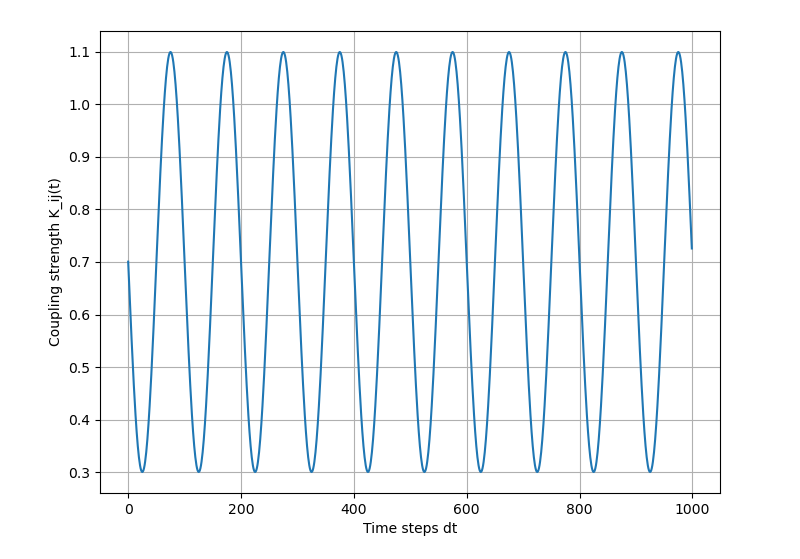
\includegraphics[width = 11cm]{Proj_fig3.png}
    \caption{\( K_{i,j}(t) \) with phase offset \( \psi_{j,i} \) 3.14 and frequency offset \( g_{i,j} \) was 1 (fast time-varying coupling strength). \( K_{i,j}(t) \) is the same for all oscillators.}
    \label{fig:3}
\end{figure}

\subsection{Common modelling parameters}

For both the models the natural frequency \(\omega_i\) was distributed according to a probability density \(g(\omega)\) as reported by \cite{Cumin} as following:
\begin{equation}
g(\omega) = 
\begin{cases} 
\frac{(1 - \omega^2)}{(\pi - 2)(1 + \omega^2)} & \text{for } |\omega| < 1 \\
0 & \text{for } |\omega| \geq 1
\end{cases}
\end{equation}

Below in figure \ref{fig:4} the probability distribution \(g(\omega)\) is illustrated.

\begin{figure}[H]
    \centering
    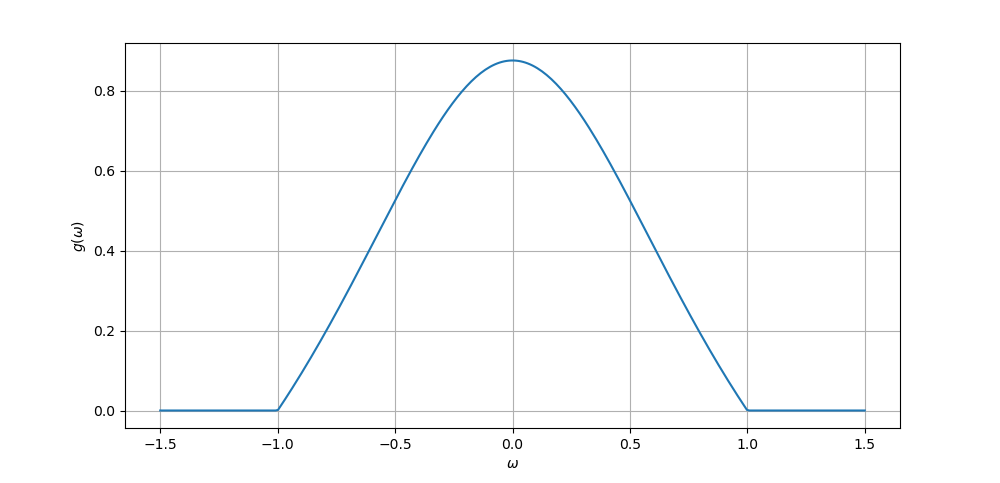
\includegraphics[width = 12cm]{G_omega.png}
    \caption{Plot of the probability distribution \(g(\omega)\).}
    \label{fig:4}
\end{figure}

Further, the order parameter \(r\) was obtained for the both simulation results as described in \cite{Cumin}:
\begin{equation}
re^{i\psi} = \frac{1}{N} \sum_{j=1}^{N} e^{i\theta_j},
\end{equation}
where \(N\) is number of oscillators, and \(\theta_j\) is the phase of oscillator \(j\).

\section{Results}

First, the order parameter as a function of time of the reproduced Kuramoto model with desynchronization was compared to corresponding results by Cumin \& Unsworth \cite{Cumin}. In Figure 4 below, it seems that four out of six visual characteristics correspond (green check marks) between the reproduced and original results, one visual characteristic did not seem to match (red x mark), and one visual characteristic could be seen to possibly remind slightly, but not enough to confirm.

\begin{figure}[H]
    \centering
    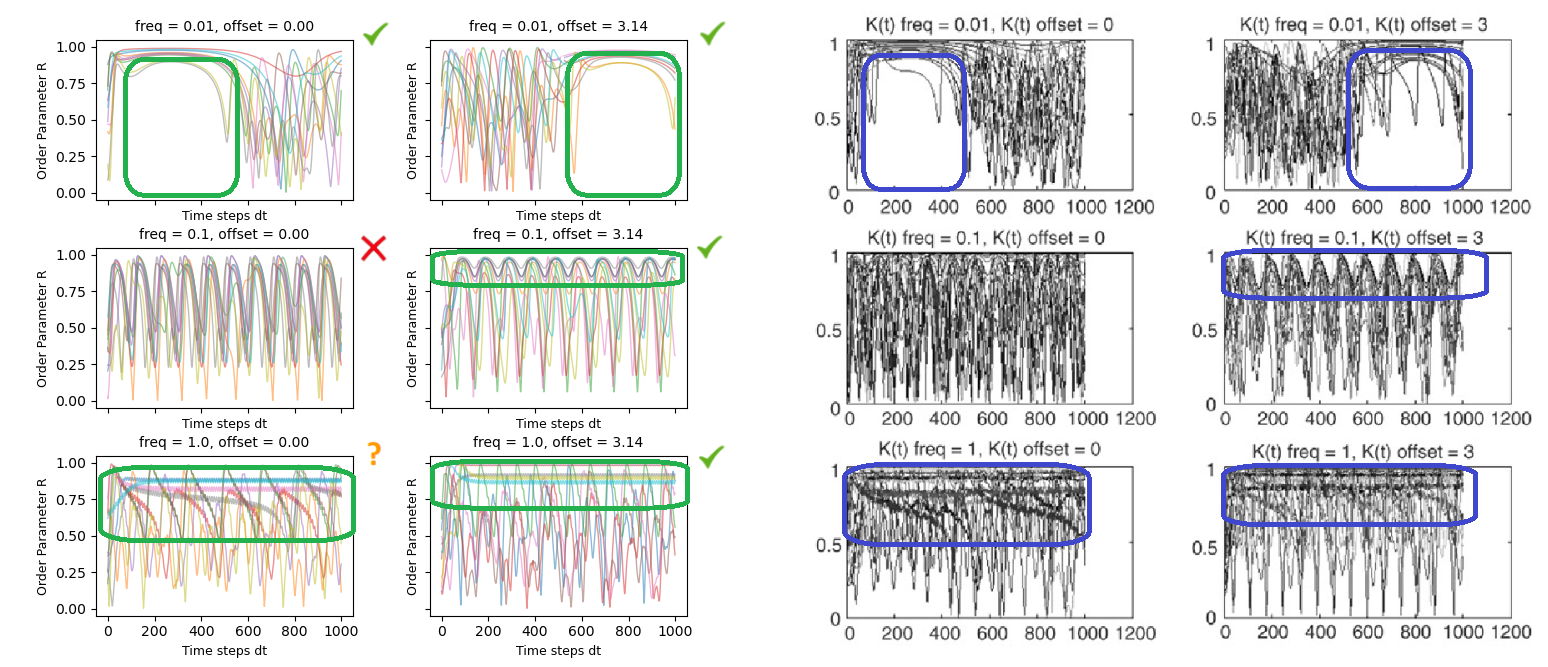
\includegraphics[width=15cm]{Proj_results.png}
    \caption{Reproduced (left) and original by Cumin \& Unsworth \cite{Cumin} (right) of order parameter as a function of time for Kuramoto model with desynchronization. Visual characteristic areas indicated with rectangles. Evaluation of visual characteristics indicated with green check mark (=similarities identified), orange question mark (=possible similarities), and red x mark (=limited similarity).}
    \label{fig:5}
\end{figure}

Next, the order parameter as a function of time was compared between the both models. In Figure \ref{fig:6} one can notice that the Kuramoto model synchronizes when the coupling strength K exceeds the critical coupling strength and that the Kuramoto model with desynchronization synchronizes and desynchronizes throughout the simulation.

\begin{figure}[H]
    \centering
    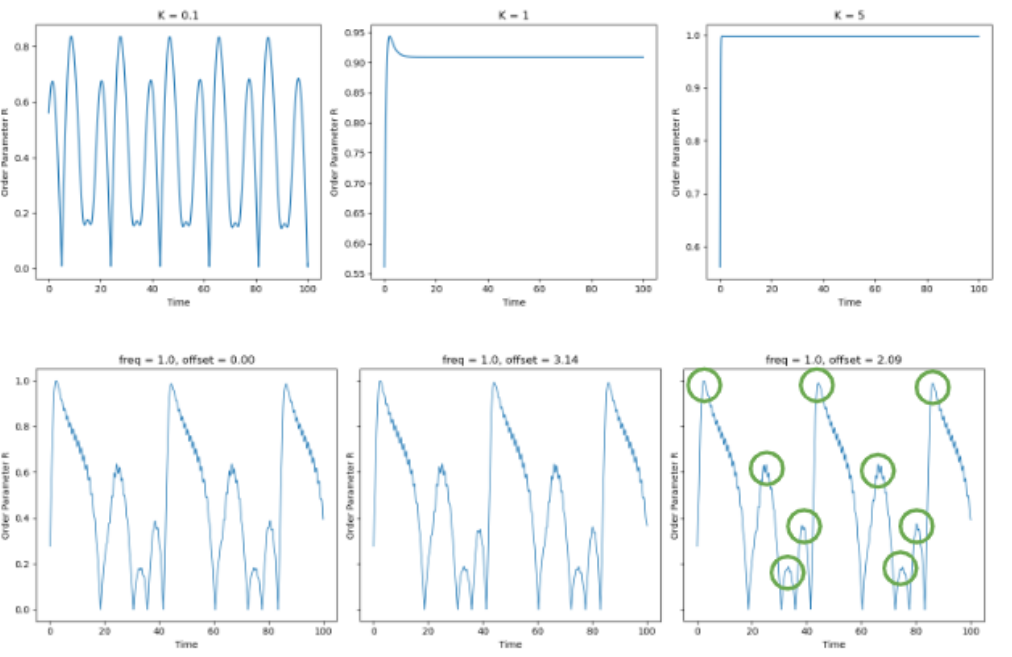
\includegraphics[width=12cm]{Proj_fig6.png}
    \caption{Order parameter as function of time for Kuramoto model (upper part) and Kuramoto model with desynchronization (lower part). In the upper part K is coupling strength. In lower part freq = 1.0 corresponds to fast time-varying coupling strength where \( g_{i,j} = 1\) and offset = [0.00, 3.14, 2.09] corresponds to phase offsets  \( \psi_{i,j} \). Peaks in the last graph are indicated with green circles.}
    \label{fig:6}
\end{figure}

\section{Discussion}
Four out of six visual characteristics of order parameter results for time-varying coupling strength Kuramoto model by \cite{Cumin} reminds of the reproduced results (Figure \ref{fig:5}). Hence it seems that this study succeeded in reproducing Kuramoto model with desynchronization.

Several peaks in the order parameter as a function of time were observed for Kuramoto with desynchronization, whereas no peaks were observed in Kuramoto model with coupling strength above the critical value (Figure \ref{fig:6}). Hence desynchronization was successfully induced into the Kuramoto model via time-varying coupling strength of 4 oscillators connected to all-to-all configuration.

This incremental study supported, to our knowledge, the restricted amount of earlier findings, that desynchronization can be induced into Kuramoto model via time-varying coupling strength. 

In our study we focused on recreating the results of \cite{Cumin} and due to a lack of available data, we had to resort to a phenomenological comparison between the resulting plots. In future work, analyzing the desynchronisation could be done in a more rigorous manner e.g. by mathematical comparison based on data from the model being compared (this assumes the models are open sourced which was not the case here).

Further studies of interest could also include testing larger systems with more oscillators and different coupling schemes.

The scientific, economic, and societal impact of this study is expected to be quite modest. The clinical relevance is also expected to be low.

Modeling of the brain is a very important tool in order to understand better how the brain operates. By creating more accurate models, more accurate treatments for severe brain disorders can be developed and very likely new disruptive applications in new areas mimicking how the brain works.  


\begin{thebibliography}{9}

\bibitem{Maistrenko}
Maistrenko, Yu \& Popovych, O \& Burylko, Oleksandr \& Tass, Peter. (2004). Mechanism of Desynchronization in the Finite-Dimensional Kuramoto Model. Physical review letters. 93. 084102. 10.1103/PhysRevLett.93.084102. 

\bibitem{Strogatz}
Strogatz, Steven. (2000). From Kuramoto to Crawford: Exploring the onset of synchronization in populations of coupled oscillators. Physica D: Nonlinear Phenomena. 143. 1-20. 10.1016/S0167-2789(00)00094-4. 

\bibitem{Han}
Han SK, Kurrer C, Kuramoto Y. Dephasing and bursting in coupled neural oscillators. Phys Rev Lett. 1995 Oct 23;75(17):3190-3193. doi: 10.1103/PhysRevLett.75.3190. PMID: 10059517.

\bibitem{Cumin}
Unsworth, C.P. \& Cumin, David. (2007). Generalising the Kuramoto Model for the study of Neuronal Synchronisation in the Brain. http://www.esc.auckland.ac.nz/research/tech/esc-tr-638.pdf. 226. 10.1016/j.physd.2006.12.004. 

\bibitem{Manos}
Manos T, Diaz-Pier S, Tass PA. Long-Term Desynchronization by Coordinated Reset Stimulation in a Neural Network Model With Synaptic and Structural Plasticity. Front Physiol. 2021 Sep 8;12:716556. doi: 10.3389/fphys.2021.716556. PMID: 34566681; PMCID: PMC8455881.

\end{thebibliography}

\end{document}
